\documentclass[12pt]{article}

\usepackage[margin=1in]{geometry}
\usepackage{graphicx}
\usepackage{amsmath}
\usepackage{float}
\usepackage{titlesec}

\begin{document}

\title{Autoencoder Ablation Study}
\maketitle

\section{Effect of Output Activation Function}

\subsection{Objective}
The objective of this ablation study is to systematically evaluate the impact of the output activation function on the performance of an Autoencoder trained on the MNIST dataset. Specifically, we compare the reconstruction quality and convergence behavior when using \textbf{Sigmoid} and \textbf{Tanh} activation functions in the final layer.

\subsection{Model Setup}

A fully connected Autoencoder architecture was made using pyTorch library
\begin{itemize}
    \item Encoder: $784 \rightarrow 128 \rightarrow 64 \rightarrow 32$ (Bottleneck)
    \item Decoder: $32 \rightarrow 64 \rightarrow 128 \rightarrow 784$ (Reconstructed Image)
\end{itemize}

The following training configuration was used:
\begin{itemize}
    \item Dataset: MNIST Dataset
    \item Input normalization: Pixel values were scaled to $[0,1]$
    \item Loss function: Mean Squared Error (MSE) (For Reconstruction)
    \item Optimizer: Adam
    \item Number of epochs: 30
\end{itemize}

Two models were trained under identical conditions, differing only in the output activation function:
\begin{itemize}
    \item \textbf{Model A:} Sigmoid activation
    \item \textbf{Model B:} Tanh activation
\end{itemize}

\subsection{Results}

\subsubsection{Reconstruction Loss Analysis}

\begin{figure}[H]
    \centering
    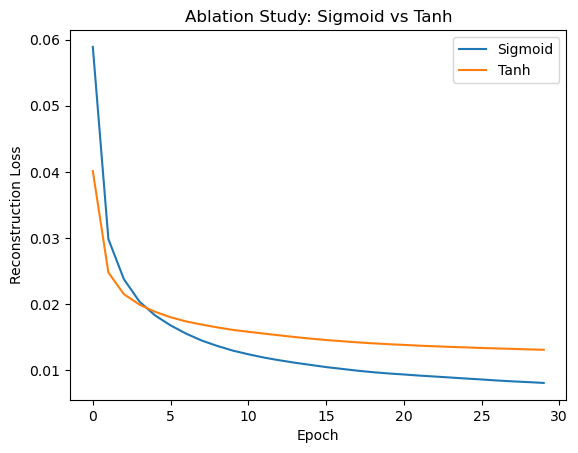
\includegraphics[width=0.7\linewidth]{plots/loss_plot.png}
    \caption{Reconstruction loss for Sigmoid and Tanh activations}
\end{figure}

From the loss curves, the following observations can be made:
\begin{itemize}
    \item Both models exhibit a decreasing trend in reconstruction loss, indicating successful learning.
    \item The Sigmoid-based model consistently achieves lower reconstruction loss throughout training.
    \item The gap between the two models increases over epochs, suggesting better convergence behavior for Sigmoid.
\end{itemize}

\subsubsection{Reconstruction Comparison}

\begin{figure}[H]
    \centering
    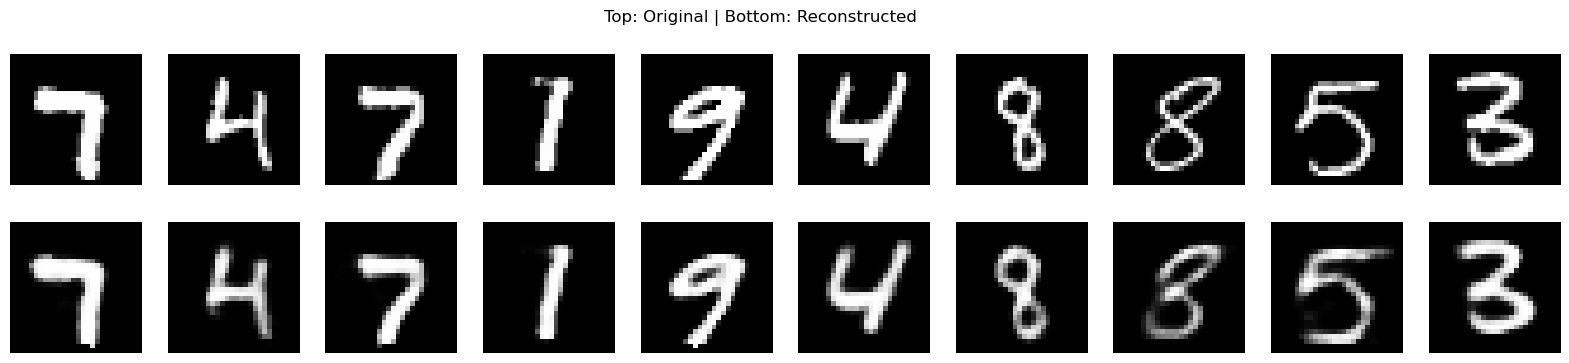
\includegraphics[width=\linewidth]{plots/sigmoid_recon.png}
    \caption{Reconstruction using Sigmoid activation }
\end{figure}

\begin{figure}[H]
    \centering
    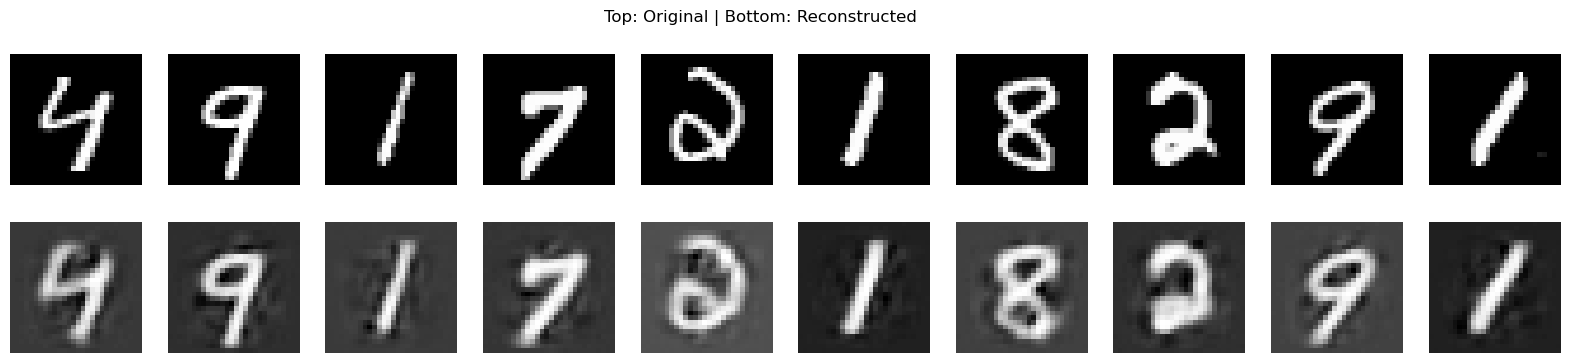
\includegraphics[width=\linewidth]{plots/tanh_recon.png}
    \caption{Reconstruction using Tanh activation }
\end{figure}

It is clearly visible that:
\begin{itemize}
    \item The Sigmoid model produces sharper and more accurate reconstructions.
    \item The Tanh model exhibits noticeable blurring and distortion.
    \item Background regions in Tanh reconstructions appear inconsistent due to negative output values.
\end{itemize}

\subsection{Discussion and Analysis}

The observed performance difference can be attributed to the inherent mismatch between the output range of the activation function and the input data distribution.\\ \\The MNIST data set is normalized such that the pixel intensities are in the range $[0,1]$. The output ranges of the activation functions are:
\begin{itemize}
    \item Sigmoid: $[0,1]$
    \item Tanh: $[-1,1]$
\end{itemize}

Thus, Sigmoid provides a direct mapping to the data distribution, whereas Tanh introduces negative values that do not naturally correspond to valid pixel intensities.\\ \\Due to this mismatch, the Tanh-based model is required to learn an additional transformation to align its output with the target distribution. This increases the complexity of the optimization problem and leads to slower convergence and higher reconstruction error

\paragraph{Visual Inconsistencies:}
The presence of negative values in Tanh outputs leads to distortions when visualized, as pixel intensities are inherently non-negative. This results in:
\begin{itemize}
    \item Blurred digit boundaries
    \item Irregular background intensities
    \item Loss of fine structural details
\end{itemize}

\subsection{Conclusion}

This ablation study demonstrates that the choice of output activation function significantly influences Autoencoder performance. When the input data is normalized to $[0,1]$, the Sigmoid activation function is more appropriate due to its compatible output range, leading to improved reconstruction quality and faster convergence.\\ \\It is important to note that if the input data were normalized to the range $[-1,1]$, the Tanh activation function would become a more suitable choice and could potentially produce comparable or improved performance.

\end{document}